\section{Principio dos trabalhos virtuais}

\begin{center}
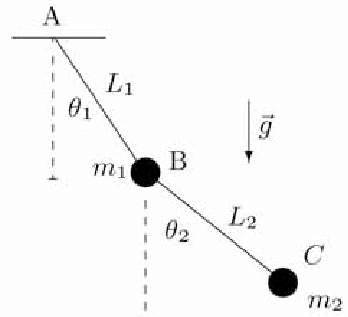
\includegraphics[width=8cm]{C:/Users/patri/Downloads/Poli/lateco/mecanica/figuras/pendulo_duplo.png}
\end{center}

\begin{namedtheorem}[Definição: Trabalho]
O \textbf{trabalho elementar} sobre uma partícula que percorre um caminho é definido como \\
$d\tau = \vec{F}\cdot d\vec{r} = \sum_{i=1}^n \vec{F_i}\cdot d\vec{r_i}$
\end{namedtheorem}

\subsection{Deslocamento Virtual}

É definido como um deslocamento de uma partícula \textit{arbitrariamente pequeno}, em conforme com os vínculos aos quais a partícula estiver sujeita. 

$\delta \vec{x} = \delta x_1 + \delta x_2 + \cdots, + x_N$

Apenas deslocamentos que não desrespeitam as equações dos vínculos são permitidos.


\subsection{Vinculos no deslocamento virtual}

Neste tipo de deslocamento, considera-se que este deslocamento é instantâneo, portanto o tempo é desconsiderado de todas equações, portanto todo vínculos se tornam \textit{esclerônomos}.

$\phi_j(x_1, x_2, \cdots, x_{N}, t) = 0, \textit{  } j =1, \cdots, k$

Diferenciando

$d \phi_j = \sum_{i=1}^{N} \frac{\partial \phi_j}{\partial x_i} + \frac{\partial \phi_j}{\partial t}dt = 0, \textit{  } j=1, \cdots, k$

No deslocamento virtual, tem-se que:

$\partial \phi_j = \sum_{i=1}^{N} \frac{\partial \phi_j}{\partial x_i}, \textit{  } j=1, \cdots, k$

Desta forma, um \textbf{deslocamento virtual}, não necessariamente pode ser convertido para um \textbf{deslocamento virtual}, caso haja algum \textbf{vínculo reônomo}

\subsection{Trabalho Virtual}

A condição \textbf{necessária e suficiente} para um sistema estar em equilibrio é que:

$\delta \tau = \sum_{i=0}^n \vec{F_i}\delta\vec{r_i} = 0 $

Tal fato é especialmente vantajoso para sistemas que há muitos agentes, dispensando o calculo de forças internas para impor condições de equilibrio.























